Besides the need to incorporate Next-Share technologies, P2P-Tube was also designed to be useful to the users. In the next subsections the usability and technical needs that governed our architecture are explained.

\subsection{Design Principles}
\label{subsec:design-principles}

P2P-Tube platform has been designed with a few basic design principles in mind:

\begin{enumerate}
 \item Provide as much as possible the \textbf{features} needed by such a platform, as they appear on similar platforms from the web.
 \item Provide to users a familiar \textbf{user interface} which resembles similar platforms from the web.
 \item Ensure that the platform \textbf{scales} well to a size of a few thousands of users.
 \item Ensure that the platform is \textbf{general purpose}.
 \item Make the platform available for \textbf{free} and distribute the code as \textbf{open-source}, encouraging community contributions.
\end{enumerate}

Being developed in academia, in University Politehnica of Bucharest, P2P-Tube was designed to fit well to our needs. The scalability requirements of a few thousands users, enumerated in Principle 3 above is enough for our Faculty of Automatic Control and Computers. However, despite this product was designed in the academia and fits its needs, we ensure that it can be generally purpose as stated in Principle 4 because of the features incorporated and its user interface tied to Principles 1 and 2.

\subsection{Features}
\label{subsec:features}

P2P-Tube provides to the users the following features:

\begin{itemize}
 \item \textbf{Categories}. Video assets can be grouped in \textit{categories} for a better organization of them.
 \item \textbf{Video plugin switching}. If the user has installed both Next-Share plugins (NextSharePC and SwarmPlayer) he is able to switch between them at any moment from the video watching page.
 \item \textbf{Users and accounts}. Users can apply for an account by registering to the site. Throughout registration, several fields can be completed, some of them mandatory, some of them optional, defining the \textit{user profile}. Authentication is possible through three methods: \textit{internal authentication}, \textit{LDAP authentication} and \textit{OpenID authentication}.
 \item \textbf{Uploading video assets}. Logged in users can upload new video assets to the site, which can be seen by others.
 \item \textbf{Social interaction}. Users can see each other's profiles, comment each other's video assets and vote them. Video assets uploaded by an user can be explored.
 \item \textbf{Searching}. Video assets can be searched by keywords and the results must be ordered by their relevance. The search can be done in the whole set of videos or in a particular category.
\end{itemize}

\textit{Internal authentication} is for users that applied for an account by the \textit{Registration} page. There are situations when the platform must be integrated with other services or sites. For example in our university we use P2P-Tube to share videos of technical presentations, courses or social events. We also have Moodle learning platform where students already have an account, so it was desired that users can authenticate on P2P-Tube we the same account credentials from Moodle. This has been achieved thorough LDAP which permits students to authenticate on both sites with the same user name and password, without requiring them to create an additional account. Another way to make users skip signing up is by using OpenID, a standard protocol which allows them to sign in through an account from another site. However, this third party site must support OpenID. So, for example, users that already have an account on Yahoo!, Google, Twitter or WordPress can securely sign in with the same user names and passwords from that accounts. When users log in for the first time using external authentication, like LDAP or OpenID, they must complete their profile.

Users can upload video assets through an upload mechanism described in the next subsection.

\subsection{Content Ingestion}
\label{subsec:content-ingestion}

NextSharePC can play any video format as long as VLC supports it and SwarmPlayer supports only video containers and codecs which are compliant with HTML5. Most modern browsers support videos having Ogg containers with Vorbis audio compression and Theora video compression or WebM containers with Vorbis audio compression and VP8 video compression. Users must be able to upload videos in a format of their choice like MPEG, DivX or AVC/H.264. Thus, the platform must perform a conversion, also known as \textit{transcoding}, from an input user format to a NextShare compliant format. P2P-Tube converts all video assets to videos with Ogg containers and Vorbis+Theora compression in order to be compatible with most modern browsers and to make video assets playable with any of the two NextShare plugins. However this can be changed from the platform configuration.

Besides video transcoding, several other operations must be performed in order to make new video assets available on the platform. This is done by a \textbf{Content Ingestion Server} (\textbf{CIS}) which is typically located on a different machine.

An user uploads a video file, referred here as \textit{raw video file}, to a web server and may also provide additional information about it, like title, description, tags etc.. When video upload is finished the process of content ingestion is started by the web server by sending a content ingestion request to a CIS. This is done directly, if the system has a single CIS, or indirectly via a CIS Load Balancer (CIS-LB), which forwards the request to one CIS from a pool of several CIS machines. By doing load balancing, the indirect request method provides scalability because more content ingestion jobs can run in parallel, allowing more users to add content simultaneously to the platform. By these means availability is also increased, the system becoming fault tolerant in case of CIS failures.

Note that sending content ingestion request is transparent for the web server. There is no difference for it if this is done directly to a CIS or indirectly through a CIS-LB. This simplifies implementation of the web server and hides the abstraction of content ingestion from it.

\begin{figure}[h]
  \begin{center}
    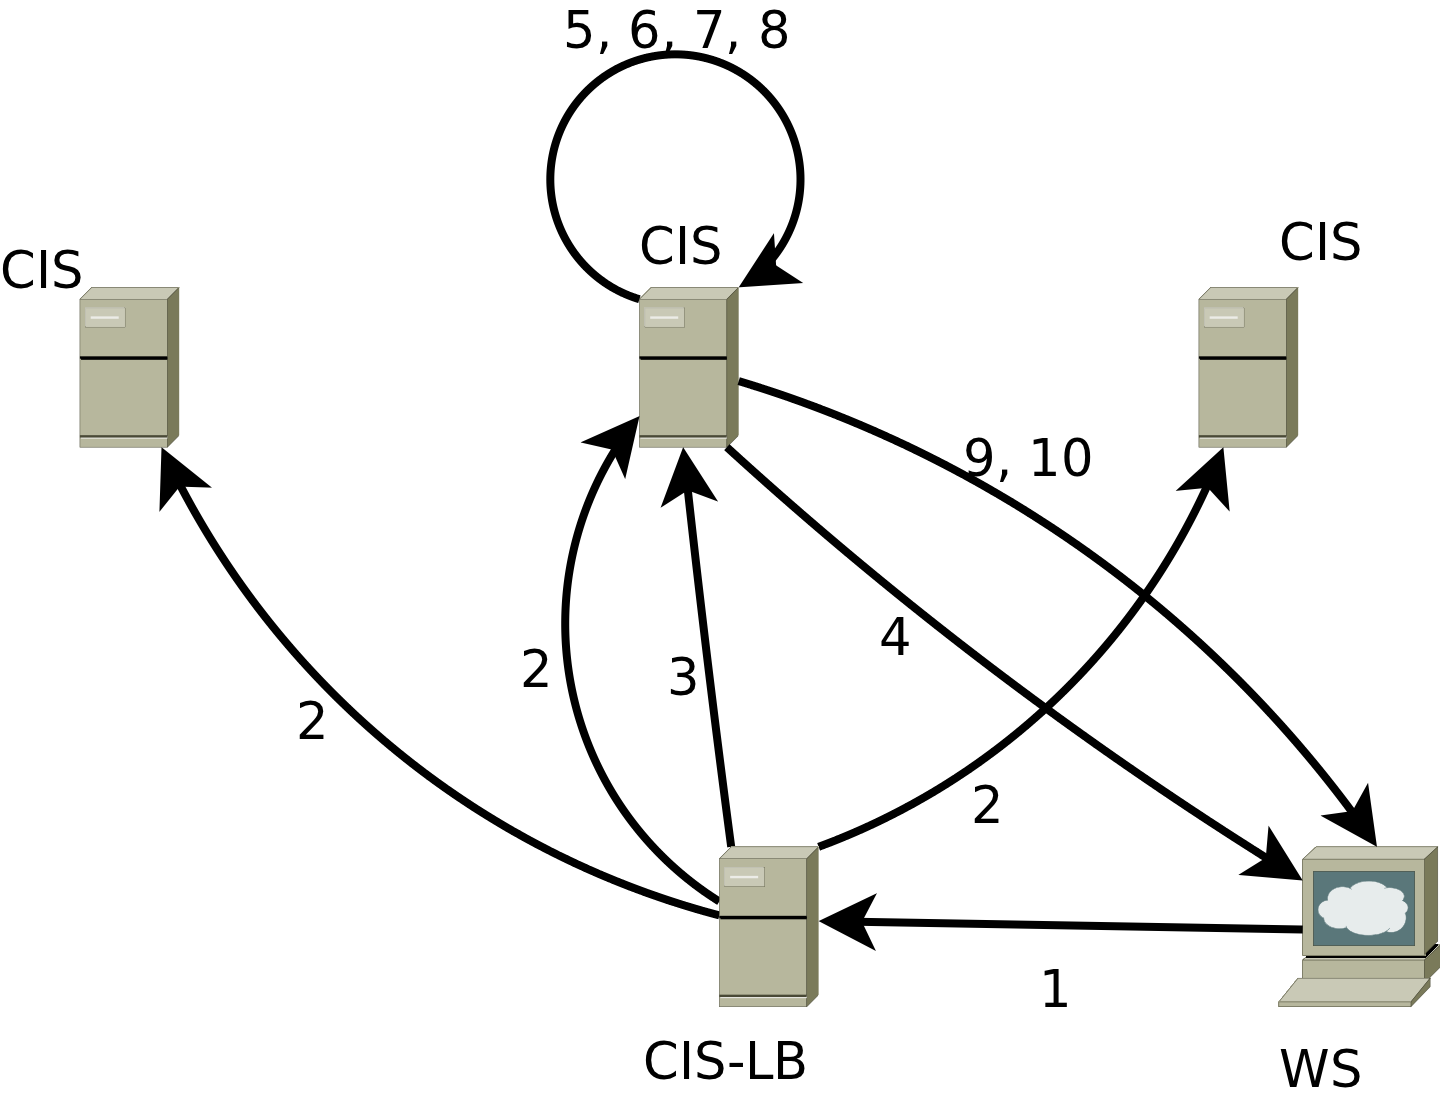
\includegraphics[width=\columnwidth]{img/content-ingestion.png}
  \end{center}
  \caption{Content Ingestion Process}
  \label{fig:content-ingestion}
\end{figure}

CIS operation through a CIS Load Balancer is described in Figure \ref{fig:content-ingestion}. Until the end of this subsection, the numbers in brackets refer to arrows from the figure. The web server sends a \textbf{content ingestion request} to CIS-LB (1), which must choose the least loaded CIS from the system. To do this it queries each CIS for its load by sending a \textbf{get load request} (2) and establishes by processing the answer which one is the least loaded. The content ingestion request previously received is then forwarded to the least loaded CIS (3), informing it about the new video file that has been uploaded. The message also contains information about one or more formats in which the video must be converted referred here as \textit{destination formats}. This information includes parameters for each format like image resolution, frame rate, audio quality etc.. The least loaded CIS which received the request executes a job on the uploaded raw video file by doing the following operations:

\begin{itemize}
 \item \textbf{Transfers locally} (4) the raw video file from the web server.
 \item \textbf{Transcodes} (5) the raw video file to one or more \textit{destination formats} resulting \textit{transcoded video files}.
 \item \textbf{Extracts image thumbnails} (6) from the raw video file.
 \item \textbf{Creates torrent files} (7) (\textit{.tstream}) for transcoded video files.
 \item \textbf{Seeds} (8) the transcoded video files by using the torrent files previously created.
 \item \textbf{Transfers back} (9) torrent files and image thumbnails to the web server.
 \item Notifies the Web Server about the \textbf{job completion} (10) so that it can make the video accessible to the users.
\end{itemize}

In the end of the content ingestion process all other Content Ingestion Servers from the system must be aware of the new torrent files in order to seed them. First of all, the new torrent files need to be locally accessible to them, so all torrent files can be shared by CIS machines on a \textit{distributed file system} such as NFS, LustreFS or GlusterFS. The overhead of using shared storage between CIS machines shouldn't affect performance, even if NFS is used, which serves files through a single machine. This is because torrent files are very small so concurrently accessing more files on the shared file system can affect performance in a negligible manner.

When the web server is notified about the job completion (10) a seed request must arrive to each CIS so that they can start seeding the new torrent files available in the distributed file system. This request is originated from the web server and there is no need to do this on a single CIS system, because this is already done in step 8 from Figure \ref{fig:content-ingestion}, so the web server can be configured to skip this redundant step from its configuration. In a multiple CIS system this step is mandatory for ensuring high availability of the new video assets. Thus, a \textbf{seed request} is sent from web server to CIS-LB, which forwards this message to all CIS from its jurisdiction. Upon reception they will start seeding requested torrent files which are located in the distributed file system.